% Created 2020-11-27 ven. 10:07
% Intended LaTeX compiler: pdflatex
\documentclass[a4paper]{article}
\usepackage[utf8]{inputenc}
\usepackage[T1]{fontenc}
\usepackage{graphicx}
\usepackage{grffile}
\usepackage{longtable}
\usepackage{wrapfig}
\usepackage{rotating}
\usepackage[normalem]{ulem}
\usepackage{amsmath}
\usepackage{textcomp}
\usepackage{amssymb}
\usepackage{capt-of}
\usepackage{natbib}
\usepackage{array}
%\usepackage{subfigure}
\usepackage{subcaption}
\usepackage[linktocpage,pdfstartview=FitH,colorlinks,
linkcolor=blue,anchorcolor=blue,
citecolor=blue,filecolor=blue,menucolor=blue,urlcolor=blue]{hyperref}
\usepackage{geometry}
\geometry{a4paper,total={170mm,257mm},left=10mm,	top=20mm,	rmargin = 20mm,	bottom = 20mm}
\usepackage{babel}
\newtheorem{theorem}{Theorem}
\newtheorem{corollary}{Corollary}
\newtheorem{lemma}[theorem]{Lemma}
\newtheorem{Proposition}{Proposition}
\newtheorem{Remark}{Remark}
\newtheorem{Assumption}{Assumption}
\newtheorem{Definition}{Definition}
\usepackage{graphicx}

\def\1{{\bf 1}_N}
\def\0{{\bf 0}}
\def\N{{\mathbb N}}
\def\R{{\mathbb R}}
\def\E{\mathcal{E}}
\def\G{\mathcal{G}}
\def\T{\mathcal{T}}
\def\I{\mathcal{I}}
\def\L{\mathcal{L}}
\def\P{\mathcal{P}}
\newcommand{\unn }{\{1,\ldots, n\}}
\newcommand{\unN}{\{1,\ldots, N\}}
%\author{Bikash Adhikari}
%\date{\today}
\title{Report: MPC with rate limitation and switching frequency minimisation} 
%\hypersetup{
% pdfauthor={Bikash Adhikari},
% pdftitle={Linear Quadratic Regulator (LQR)},
% pdfkeywords={},
% pdfsubject={},
% pdfcreator={Emacs 26.3 (Org mode 9.3.6)}, 
% pdflang={English}}


\begin{document}
\newpage
\maketitle
% \tableofcontents

% \newpage
\section{Quantisation}
Let $w \in \mathbb{R}$ be the input, $\mathbf{Q}$ be the quantiser and $y \in \mathbb{U}$ the quantiser output, as shown in the additive model of quantisation in the Figure \ref{fig:quan_add_model}.  Let us define the quantisation error as 
\begin{equation}
	q = \mathbf{Q}(w) - w= y -w.
	\label{eq:error}
\end{equation}
\begin{figure}[!htb]
    \centering
    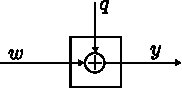
\includegraphics[scale = 1]{figures/quantizer_additive_model.pdf}
    \caption{Quantiser additive model}
    \label{fig:quan_add_model}
\end{figure}
The quantisation requires the signal to be mapped to a finite signal where each value of the output $y$ is restriced to belong to a finite set $\mathbb{U}$. The elements of the set $\mathbb{U}$ represent the quantiser levels and depends on the word-size of the quantiser. 

\section{Noise and Distortion in the DACs.}
\subsection{Slewing Distortion}
Slew rate defined as the maximum rate of change of output voltage level. In other words, it referes to how fast the DAC is capable of changing its output voltage in response to a change in input. 
An ideal DAC creates an output voltage that is instantaneously proportional to the input number which is not possible in practice due to temporal limitations.  If the input number to the DAC change from one value another at time $t_{1}$, the output voltage reaches new value at time later than time $t_{1}$. This is one of the most common distortions in DACs and is governed in large part by the slewing of the output amplifier and its compensation in physical DACs and shown in the following figure. 
\begin{figure}[!ht]
	\centering
		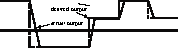
\includegraphics[scale = 2.5]{figures/effectofslew.pdf}
		\caption{Effect of slew limiting on the output of the DAC}
		\label{fig:slew1}
\end{figure}
\begin{figure}[!ht]
	\centering
		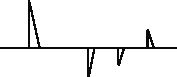
\includegraphics[scale = 2.5]{figures/slewlimitederror.pdf}
		\caption{Slew limited error}
		\label{fig:slew2}
\end{figure}
\section{Moving horizon optimal quantiser (MHOQ)}
The design criteria for the MHOQ is the minimization of the perceived errors defined as follows:
\begin{equation}
	e(t) = H(z)(w(t)-y(t))
	\label{eq:error1}
\end{equation}
where  $H(z)$  is  a stable time-invariant linear low-pass filter with the following state-space
\begin{equation}
	\label{eq:filter_statespace}
	H(z) = 1 + C(z I - A)^{-1} B
\end{equation}
The error $e$  then can be written as the output of the following state-space representation of $H$
\begin{equation}
	\begin{aligned}
		x(t+1) &= A x(t) + B (w(t)-y(t))		\\
		e(t) &= Cx(t) + w(t)-y(t)
	\end{aligned}
	\label{eq:statespace1}
\end{equation}
where $x \in \mathbb{R}^{n}$ is the state vector.  The error $e$ corresponds to the difference between the filtered quantised signal and the filtered input signal. 

For moving horison implementation, the optimisation problem is defined as the problem of finding $y \in \mathbb{U}$ that minimises  the cost function  while satisfying the state equations as follows:
\subsection{Mixed Integer Quadratic Optimisation Problem}
\begin{align}
		& y^{\ast}(t) = \arg  \min_{y(t) }	V_{N}  = \sum_{t=k}^{k+N-1} e^{2}(t) \label{eq:optobj1}\\
		\intertext{subject to}
		&x(t+1) = A x(t) + B (w(t)-y(t))	\label{eq:optconst1}	\\
		&e(t) = Cx(t) + w(t)-y(t)	\label{eq:optconst2}	\\
		&y(t) \in \mathbb{U}. \label{eq:optconst3}
	\end{align}
\subsection{Mixed Integer (Binary) Quadratic Optimisation Problem}
The optimization problem \eqref{eq:optobj1}-\eqref{eq:optconst3} can be reformulated as an optimization problem with the binary variables. Let $\mathcal{B}$ be the number of bits.  $b_{i} = \{0,1\}$ and $Q_{i}$ $, i = \{0, 1, \ldots, 2^{\mathcal{B}}-1\}$, be the binary variables and quantisation levels, respectively. 
\begin{align}
		& y^{\ast}(t) = \arg  \min_{y(t) }	V_{N}  = \sum_{t=k}^{k+N-1} e^{2}(t) \label{eq:optobj12}\\
		\intertext{subject to}
		&x(t+1) = A x(t) + B (w(t)-y(t))	\label{eq:optconst12}	\\
		&e(t) = Cx(t) + (w(t)-y(t))	\label{eq:optconst22}	\\
		&y(t) = \sum_{i = 0}^{2^{\mathcal{B}}-1} Q_{i}b_{i}, \quad \sum_{i = 0}^{2^{\mathcal{B}}-1}b_{i}  =1, \quad b_{i} = \{0,1\}. \label{eq:optconst32} 
	\end{align}


\section{MPC with Switching Frequency Minimization}
The  amount of the states that switches at each sampling time can be minimised by penalising the total number of switched with some weighting factor.  Two control objective are achieved in the propose algorithm, optimal quantisation and switching frequency minimisation. The minimised switching frequency leads to the mitigation of the distortion in the output signal due to slewing effectin the DACs.   The optimisation problem is as follows,  
\begin{align}
		& y^{\ast}(t) = \arg  \min_{y(t) }	V_{N}  = \sum_{t=k}^{k+N-1} e^{2}(t) + \beta \mathcal{N}_{s}\label{eq:optobj121}\\
		\intertext{subject to}
		&x(t+1) = A x(t) + B (w(t)-y(t))	\label{eq:optconst122}	\\
		&e(t) = Cx(t) + (w(t)-y(t))	\label{eq:optconst223}	\\
		&y(t) = \sum_{i = 0}^{2^{\mathcal{B}}-1} Q_{i}b_{i}(t), \quad \sum_{i = 0}^{2^{\mathcal{B}}-1}b_{i}(t)  =1, \quad b_{i} = \{0,1\}^{N}. \label{eq:optconst324} \\
		&\mathcal{N}_{s} = \sum_{i = 0}^{2^{\mathcal{B}}-1} |b_{i}(t) - b_{i}(t-1)|^{2}
	\end{align}
	where $b_{i}(t-1)$ is the state of the switch $i$ at the previous state and $b_{i}(t)$ is the sate of switch $i$ at the current state and $\beta$ is the weighting factor.  The average switching frequency of the coverters is defined as follows 
	\begin{equation}
		f_{sw} :=  \frac{1}{M T_{s}} \sum_{i = 1}^{M} \|\Delta b_{i}\|_{1}
	\end{equation}
	where $M$ is the total number of samples, $T_{s}$ is the sampling rate and $\Delta b_{i} = b_{i} - b_{i-1}$.

% \begin{table}[thb]
% 	\centering
% \caption{ DAC-Ideal:Simulation Results: Carrier Frequency $ 999 Hz$}
% 	\begin{tabular}{ | c |c|c|c|c|c|c|c|c|c|c|} 
% 	  \hline
% 	  $\beta$& 0 & 0.0001 & 0.00025 &0.0005  & 0.00075 & 0.001  & 0.0025 & 0.005 & 0.0075 & 0.01 \\ 
% 	  \hline
% 	  ENOB & 8.39 & 8.08 & 7.72 & 7.39 & 6.96  & 6.69 & 6.01  & 5.51  & 5.37 & 5.14 \\ 
% 	  \hline
% 	  $f_{sw} (kHz)$  & 480 & 396 & 254 & 218 & 272 & 310 & 222.2 & 236  & 223 & 201 \\ 
% 	  \hline
% 	\end{tabular}
% \end{table}

% \begin{table}[thb]
% 	\centering
% \caption{DAC-INL: Simulation Results: Carrier Frequency $ 999 Hz$}
% 	\begin{tabular}{ | c |c|c|c|c|c|c|c|c|c|c|} 
% 	  \hline
% 	  $\beta$& 0 & 0.0001 & 0.00025 &0.0005  & 0.00075 & 0.001  & 0.0025 & 0.005 & 0.0075 & 0.01 \\ 
% 	  \hline
% 	  ENOB & 7.96 & 7.73 & 7.53 & 7.28 & 6.88  & 6.68 & 6.11  & 5.55  & 5.29 & 5.13 \\ 
% 	  \hline
% 	  $f_{sw} (kHz)$  & 475 & 379 & 270 & 278 & 304 & 303 & 278 & 249  & 245 & 229 \\ 
% 	  \hline
% 	\end{tabular}
% \end{table}


\begin{figure}[!h]
	\centering
	\begin{minipage}{0.45\linewidth}
		\centering
		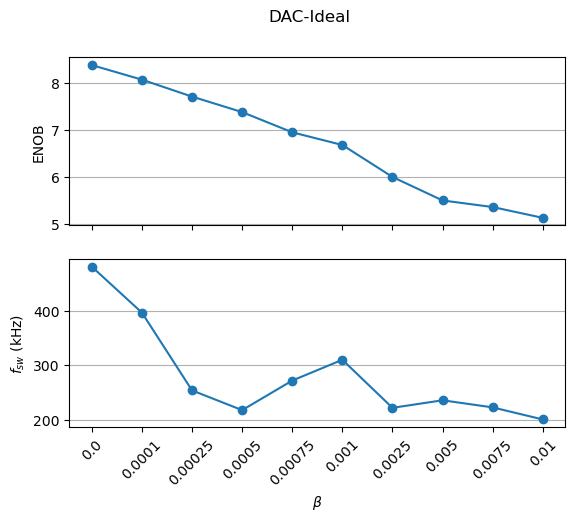
\includegraphics[scale = 0.55]{switch_plots/dac_ideal.png}
		\caption{DAC-Ideal: Effect of switching frequency $\beta$ on average switching frequency $f_{sw}$ and ENOB.}
        \label{fig:fmin_dacideal}
	\end{minipage}
	\hfil
	\begin{minipage}{0.45\linewidth}
		\centering
		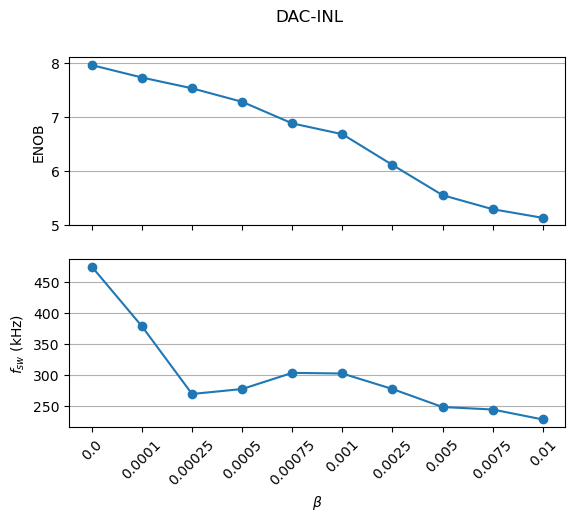
\includegraphics[scale = 0.55]{switch_plots/dac_inl.png}
		\caption{DAC-INL: Effect of switching frequency $\beta$ on average switching frequency $f_{sw}$ and ENOB.}
   \label{fig:fmin_dacinl}
	\end{minipage}
\end{figure}


\clearpage
\section{MPC with switching rate limitation:}
The MPC formulation with the rate limitation is as follows:
\begin{align}
	& y^{\ast}(t) = \arg  \min_{y(t) }	V_{N}  = \sum_{t=k}^{k+N-1} e^{2}(t) \label{eq:optobjrl1}\\
	\intertext{subject to}
	&x(t+1) = A x(t) + B (w(t)-y(t))	\label{eq:optconstrl1}	\\
	&e(t) = Cx(t) + w(t)-y(t)	\label{eq:optconstrl2}	\\
	& - L_{r} \Delta t \leq \Delta y(t) \leq L_{r} \Delta t \label{eq:optconstrl13} \\
	&y(t) \in \mathbb{U}. \label{eq:optconstrl4} 
\end{align}
The rate limitation is imposed by the constraint \eqref{eq:optconstrl13}  where $\Delta y (t) = y(t) - y(t-\Delta t) $ and the constraint \eqref{eq:optconstrl13} can be further simplifed as 
\begin{align*}	
&\Delta y(t) \leq  L_{r}\Delta t\\
&- \Delta y(t) \leq  L_{r} \Delta t
\end{align*}
Here $\Delta t = T_{s}$ and the rate limitation $L_{r}$ are assumed to constant for all sampling instants. 
\subsection*{Simulations results:}
\begin{table}[thb]
	\centering
\caption{Simulation Results: Carrier Frequency $ 999 Hz$, Total number of samples: 21021.}
	\begin{tabular}{ | m{3cm} | m{1.8cm}| m{1.8cm} | m{1.8cm}| m{1.8cm} |m{1.8cm}| m{1.8cm} |m{1.8cm}| } 
	  \hline
	  Rate limit ($L_{r} \Delta t$)& N/A & 1e6 & - & - & - & -  & -\\ 
	  \hline
	  ENOB (99Hz) & 9.444 & 4.18 & - & - & - & - & -\\ 
	  \hline
	\end{tabular}
\end{table}

\begin{figure}[!h]
	\centering
	\begin{minipage}{0.45\linewidth}
		\centering
		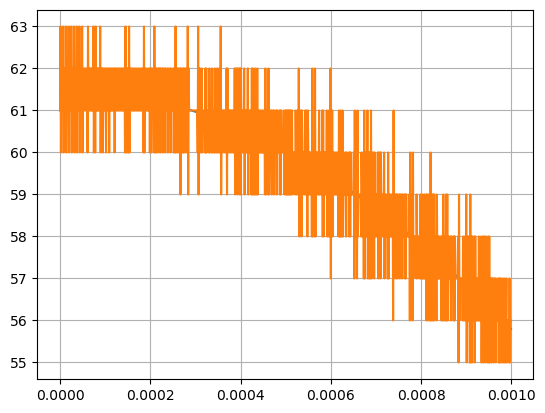
\includegraphics[scale = 0.58]{SIM_ratelimit/99Hz/No_RL_Ts_1000s.png}
		\caption{No rate limit. Carrier frequency: $99 Hz$.}
        \label{fig:direct_psd}
	\end{minipage}
	\hfil
	\begin{minipage}{0.45\linewidth}
		\centering
		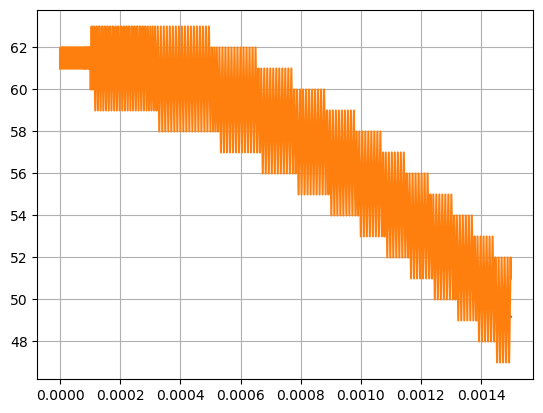
\includegraphics[scale = 0.6]{SIM_ratelimit/99Hz/RL_1e6_Ts_ALLs.png}
		\caption{Carrier frequency: $999 Hz, \beta = 100$}
   \label{fig:dsm_psd}
	\end{minipage}
\end{figure}




\end{document}